\documentclass[12pt]{report}
\usepackage[top=23mm,bottom=23mm,left=23mm,right=23mm]{geometry}
\usepackage{fancyhdr, lastpage}
\usepackage{times}
\usepackage{cite}
\usepackage{chapterbib}
\usepackage[sectionbib]{natbib}
\bibpunct{(}{)}{;}{a}{,}{,}
\usepackage[pdftex]{graphicx}
\usepackage{epstopdf}
\usepackage{subfigure}
\usepackage[footnotesize, bf]{caption}
\usepackage{amsmath}
\usepackage{amssymb}
\usepackage{setspace}
\usepackage[small,compact]{titlesec}
\usepackage{multicol}
\usepackage{multirow}
\usepackage{wrapfig}
\usepackage{minitoc}
\usepackage{array}
\usepackage{tikz}
\usepackage{enumerate}  % for enumerating with a), b) etc...
\usepackage{caption}    % for having enumertion in a caption 
\usepackage{cleveref}   % So multiple references will auto format themself
\usepackage[]{algorithm2e}


%Folder paths that contain graphics
\graphicspath{{./}
{Chapters/ConvergenceFigures/}
{Chapters/IterationsFigures/}
{Chapters/MethodFigures/}
{Chapters/ModelFigures/}
{Chapters/Show1DFigures/}
{Chapters/Typical_SimulationFigures/}}


% PDF hyper-linking (set colors to black for printing)
%\usepackage[ps2pdf=true,colorlinks]{hyperref}
%\usepackage[figure,table]{hypcap}
%\hypersetup{
%	bookmarksnumbered,
%	pdfstartview={FitH},
%	citecolor={black},
%	linkcolor={black},
%	urlcolor={black},
%	pdfpagemode={UseOutlines}
%}

\pdfinfo{
/Author (Eric M. Jalbert, 2014)
/Title (Numerical Analysis of Methods for Simulating Clostridium Thermocellum)
/Subject (Numerical Analysis of Methods for Simulating Clostridium Thermocellum)
}

%Paragraph symmetries...
\setlength{\parskip}{10pt}
\setlength{\parindent}{0pt}
\setlength{\parsep}{0pt}


\setcounter{secnumdepth}{5}
\setcounter{tocdepth}{1}
\renewcommand{\mtctitle}{ }
\renewcommand{\mlftitle}{ List of Figures in Chapter }
\setcounter{minitocdepth}{1}
%\setcounter{minilofdepth}{2}
\renewcommand{\abstractname}{\Large ABSTRACT}
\renewcommand{\bibname}{References}
%\renewcommand\bibsection{}
%\renewcommand{\bibsep}{0pt}

\fancypagestyle{custom}{
\lhead{\textit{E.Jalbert, 2014}}
\rhead{\textit{NUMERICAL ANALYSIS SIMULATING C.THERMOCELLUM}}
}

\fancypagestyle{References}{
\lhead{}
\rhead{\textit{REFERENCES}}
}

%%%%%%%%% If I have appendies, add the fancy page styles 
%%%%%%%%% like the example below
%\fancypagestyle{AppendixA}{
%\lhead{}
%\rhead{\textit{APPENDIX A: Default Simulation Parameters}}
%}

\begin{document}

%PreliminarySections
\pagenumbering{roman}
\input{Prelims/TitlePage}
%%Abstract
%\phantomsection
\addcontentsline{toc}{section}{Abstract}
%\section*{ABSTRACT}
\begin{abstract}
\setcounter{page}{2}
\begin{center}
%\vspace*{33pt}
\large{\textbf{Comparison of a Semi-Implicit and a Fully-Implicit Time Integration Method for a Highly Degenerate Diffusion-Reaction Equation Coupled with and Ordinary Differential Equation}}\\
\vspace*{20pt}
\begin{minipage}{0.49\textwidth}
\begin{flushleft}
\normalsize{Eric M. Jalbert}\\
\normalsize{University of Guelph,2015}
\end{flushleft}
\end{minipage}
\begin{minipage}{0.49\textwidth}
\begin{flushright}
\normalsize{Advisor}\\
\normalsize{Professor Hermann J. Eberl}
\end{flushright}
\end{minipage}
\end{center}
\vspace*{20pt}

A certain class of highly degenerate diffusion equations arises when modelling biofilm growth and propagations.
We focus on the cellulolytic \textit{Clostridium thermocellum}, because of its potential in the field of energy biotechnology.
From this system a spatially implicit model was proposed in the literature before.
Here we study a spatially explicit model.
In contrast to other biofilm systems, a special feature of this system is that the growth promoting nutrient is not diffusive but bound in the substratum on which the biofilm grows.
As a consequence one obtains a highly degenerate diffusion-reaction equation for the bacteria that is coupled to an ordinary differential equation for nutrients.
The degeneracy of the biomass equation introduces gradient blow-up at the interface which makes numerical treatment difficult.
For this, a fully-implicit time integration method is formulated so that it generalises a previously used semi-implicit method to solve the problem with increased accuracy.
The fully-implicit method uses, at each time-step, a fixed-point iteration to solve the arising nonlinear algebraic equation and can be controlled by the required tolerance for convergence.

This method is validated and tested to investigate numerous issues that arise with numerical computations: mass conservations, preservation of symmetries in the initial data, and convergence with respect to grid refinement.
Furthermore, a difference is quantified between the fully-implicit and the simpler semi-implicit methods which it generalises.
The trade-off between improved accuracy and increased computational effort is found to be optimal for tolerances that force a single extra iteration of the fully-implicit method.

The numerical method is then used to simulate \textit{C.thermocellum} biofilm formation on cellulose sheets with the main objectives of (i) understanding patterns of biofilm formation and (ii) understanding how including the spatial diffusion terms in the biomass affect the results of the simulations at a reactor-scale.
Our simulation results strongly suggest the formation of travelling wave solutions that describe how the biofilm moves across the substratum.
To test the effect of the spatial effects on overall biofilm performance, two extremes of initial biomass distributions were simulated.
A quantitative difference between the behaviour in both cases is found, but not a qualitative one.
This suggests that in applications where spatial heterogeneity is important then a two dimensional spatially explicit model that includes the spatial diffusion must be used instead of the earlier, simple spatially implicit reactor-scale ordinary differential equation model that consolidated the spatial effects with a carrying capacity on the growth term.
\end{abstract}


\setcounter{page}{3}
%\input{Prelims/Dedication}
%\input{Prelims/Acknowledgements}
%%\dominitoc
\dominilof
\setlength{\parskip}{0ex plus 0.5ex minus 0.2ex}

\tableofcontents
\pagebreak
\addcontentsline{toc}{section}{List of Figures}
\listoffigures
%\listoftables
\setlength{\parskip}{10pt}


%%%Main Texts
\pagebreak
\pagestyle{fancy}
\pagenumbering{arabic}
\doublespacing
%\onehalfspacing

\chapter{Introductions}
In here will be a bunch of info on the literature of biofilm simulations, and probably should mention the cellular automata model of C.Thermocellum in here and how this is mainly trying to make a continuous model of that simulation. 

Add also how that the existance of a travelling wave solution will be looked for, but not proven.... and how we will also try to model the growth of C.thermocellum based on the production of CO2. 

\chapter{Numerics}
\section{Model}

\begin{verbatim}
Talk about: the origins of the model (Hermann?) 
            the origins for the functions D(M), F(C,M) and G(C,M). 
            the parameters and where their values come from. 
            More....?
\end{verbatim}

The model used for simulations is based on the deterministic model developed in \cite{eberl2001deterministic} to model the development of spatially heterogenous biofilm structures. They modelled the biomass density and nutrient concentration as a two PDE-coupled system. Here the spatial diffusion of the nutrient concetration is removed to mimic the carbon substrait that C.Thermocellum consumes to grow. The PDE-ODE-coupled system is purposed as,
  \begin{align} 
     M_\tau &= \nabla_\chi \left(  \overline{D}(M) \nabla_\chi M \right) + \overline{f}(\overline{C},M) M \label{equ:model_Mtau}\\
     \overline{C}_\tau &= -\overline{g}(\overline{C}) M \label{equ:model_Ctau}
  \end{align}
where
  \begin{equation} \label{equ:model_barD}
    \overline{D}(M) = \overline{\delta} \frac{M^\alpha}{(1-M)^\beta}
  \end{equation}
  \begin{equation} \label{equ:model_barf}
   % \overline{f}(\overline{C},M) = \overline{g}(\overline{C}) - \frac{y}{10} 
    \overline{f}(\overline{C},M) = \frac{\overline{\mu} \overline{C}}{\overline{k} + \overline{C}} \left(1 - \left( \frac{M}{\overline{C}} M_0 \right)^\gamma \right) \\
  \end{equation}
  \begin{equation} \label{equ:model_barg}
    \overline{g}(\overline{C}) = \frac{\overline{y} \overline{C}}{\overline{k} + \overline{C}}
  \end{equation}
Here in (\ref{equ:model_Mtau}) the spatial diffusion of biomass is density dependent diffusion, given by (\ref{equ:model_barD}), and the growth rate of biomass, $\overline{f}(\overline{C},M)$, is given by (\ref{equ:model_barf}). The growth rate is Monod kinetic growth multiplied by logistic growth to enforce a carrying capacity and death rate in the biomass. In (\ref{equ:model_Ctau}) there is only a consumption term from the bacteria consuming the carbon substrait. 
  
  
  
  
  The dimensions of the parameters and variables are in Tabel \ref{tab:varDimensions}.
  
  \begin{table}[!hbt]
    \centering
    \begin{tabular}{|c | l | l|}
      \hline 
      Variable/Parameter & Dimensions & Parameter Value\\
      \hline 
      $\tau$ & [$days$] & $-$ \\
      $\chi$ & [$meters$] & $-$ \\
      $ M  $ & [$-$] & $-$\\
      $ C  $ & [$\frac{grams}{meters^3}$]  & $-$\\
      $ \overline{\delta} $ & [$\frac{meters^2}{days}$] & $10^{-12}$ \\
      $ \alpha $ & [$-$] & $4$\\
      $ \beta  $ & [$-$] & $4$\\
      $ \overline{\mu}$ & [$days^{-1} $] & $6$ \\
      $ \overline{k}  $ & [$\frac{grams}{meters^3}$] & $4$ \\
      $ \gamma $ & [$-$] & $0.5$\\
      $ \overline{\nu}$ & [$\frac{grams}{meters^3 \cdot days}$] & $\frac{\mu M_0}{0.63}$ \\
      $ M_0 $ & [$-$] & $10000$ \\
      $ C_0 $ & [$\frac{grams}{meters^3}$]  & $30$ \\
      \hline
    \end{tabular}
    \caption{List of parameters and their dimensions}
        \label{tab:varDimensions}
  \end{table}
  
\section {Nondimensionalization}
  For this system, it is better to nondimensionalize. To do this, the following variable changes are used:
  \begin{align}
    x &= \frac{\chi}{L} \implies L dx = d\chi\\
    t &= \mu \tau \implies \frac{1}{\mu} dt= d\tau\\
    C &= \frac{\overline{C}}{C_0} \\
    \delta &= \frac{1}{\mu L^2} \overline{\delta} \\
    k &= \frac{\overline{k}}{C_0} \\
    \nu &= \frac{\overline{\nu}}{\mu C_0} \\
    \mu &= \overline{\mu}
  \end{align}
  This gives the system
  \begin{align}
    M_t &= \frac{1}{\mu L^2} \nabla_x \left(\hat{D}(m) \nabla_x M \right) + \frac{1}{\mu} \hat{f}(C,M) \\
    C_t &= \frac{ -1}{C_0 \mu} \hat{g}(C,M)
  \end{align}
  
  where 
  \begin{equation}
    \hat{D}(M) = {\mu L^2 \delta} \frac{M^\alpha}{(1-M)^\beta}
  \end{equation}
  
  \begin{equation}
    \hat{f}({C},M) = \frac{{\mu} {C C_0}}{{k C_0} + {C C_0}} M \left(1 - \left( \frac{M}{{C}} \frac{M_0}{C_0} \right)^\gamma \right) \\
  \end{equation}
  
  \begin{equation}
    \hat{g}({C},M) = -\frac{{\mu C_0 \nu} {C C_0}}{{k C_0} + {C C_0}} M \\
  \end{equation}
  
  This can be greatly simplified by cancelling out parameters.
  
  \begin{align}
    M_t &= \nabla_x \left( {\delta} \frac{M^\alpha}{(1-M)^\beta} \nabla_x M\right) + \frac{ C }{{k } + {C}} M \left(1 - \left( \frac{M}{{C}} \frac{M_0}{C_0} \right)^\gamma \right) \\
    C_t &= - \frac{\nu C}{k + C} M
  \end{align}
  
  Now we can name functions and get the final nondimensionalized system.
  
  \begin{align} \label{equ:model_system}
    M_t &= \nabla_x \left( D(M) \nabla_x M \right) + f(C,M) \\
    C_t &= - g(C,M) 
  \end{align}
  
  where
  
  \begin{equation}
  \begin{aligned} \label{equ:model_functions}
    D(M) &= \delta \frac{M^\alpha}{(1 - M)^\beta} \\
    f(C,M) &= \frac{ C }{{k } + {C}} M \left(1 - \left( \frac{M}{{C}} \frac{M_0}{C_0} \right)^\gamma \right) \\
    g(C,M) &= \frac{\nu C}{k +C} M
  \end{aligned}
  \end{equation}
  
  with parameter values
  
  \begin{equation}
    \begin{aligned}
      L &= 0.01 m \\
      C_0 &= 30 \frac{g}{m^3} \\
      M_0 &= 1.000 \times 10^{4}\frac{g}{m^3} \\
      \delta &= 1.667 \times 10^{-9}\\
      k &= 0.1333 \times 10^{-1}\\
      \nu &= 5.291 \times 10^{2}\\
    \end{aligned}
  \end{equation}



\section{Methods}

Describe the method of solveing. Use MATH6020 project description as a baseline (since its mainly the same method).
Should give enough detail so that this method can be replicated (verbatim psuedo code?).
essentially describing the discritization of M so that it can be solved using finite difference method and how C is solved by trapezidral rule.


%%%%%%%%%%%%%%%%%%%%%%%%%%%%%%%%%%%%%%%%%%%%
\subsection{Substrate Concentration}
  The substrate concentration is represented by the following equation:
  \begin{equation} \label{eq:c=g}
    C_t = g(C,M).
  \end{equation}
  For our case we will use
  \begin{equation} \label{func:g}
    g(C,M) = -\frac{\nu C}{k + C} M.
  \end{equation}
  
  To solve for C we first apply the Fundemental Theorem of Calculus and the Trapizoidal Rule to (\ref{eq:c=g}).
  \begin{equation}
  \begin{aligned}
    \int^{t_{n+1}}_{t_n} C_t dt &= \int^{t_{n+1}}_{t_n} g(C,M) dt \\
    C_{t_{n+1}} - C_{t_n} &= \frac{(t_{n+1} - t_n)}{2} \left( g(C_{t_{n+1}},M_{t_{n+1}}) + g(C_{t_n}, M_{t_n})  \right).
  \end{aligned}
  \end{equation}
  For convience we will henceforth let $C_n = C_{t_n}$, $M_n = M_{t_n}$, and $h = t_{n+1} - t_n$.
  Now we substituite (\ref{func:g}) and try to solve explicitly for $C_{n+1}$
  \begin{equation} \begin{aligned}
    C_{n+1} - C_n &= \frac{h}{2}  \left( -\frac{\nu C_{n+1}}{k + C_{n+1}} M_{n+1}  -\frac{\nu C_n}{k + C_n} M_n \right) \\
    C_{n+1} (k + C_{n+1}) - C_n (k + C_{n+1}) &= -\frac{h}{2} \nu M_{n+1} C_{n+1} - \frac{h}{2} \frac{\nu C_n M_n}{k + C_n} (k + C_{n+1})
  \end{aligned} \end{equation}
  This gives us the following quadratic equation
  \begin{equation}  
    C_{n+1}^2 + \left( k - C_n + \frac{h}{2} \nu M_{n+1} + \frac{h}{2}\frac{\nu C_n M_n}{k + C_n} \right) C_{n+1} + \left( -k C_n + \frac{h}{2} \frac{\nu k C_n M_n}{k + C_n} \right) = 0
  \end{equation}
  from which we can identify
  \begin{equation} \begin{aligned} \label{para:abc}
    a &= 1\\
    b &= k - C_n + \frac{h}{2} \nu M_{n+1} + \frac{h}{2}\frac{\nu C_n M_n}{k + C_n}\\
    c &= -k C_n + \frac{h}{2}\frac{\nu k C_n M_n}{k + C_n}
  \end{aligned}  \end{equation}
  
  We can now solve for $C_{n+1}$ using the quadratic formula
  \begin{equation} \label{eq:Cquad}
    C_{n+1} = \frac{-b \pm \sqrt{b^2 - 4ac}}{2a}
  \end{equation}
  
  To figure out which value of $C_{n+1}$ we use, we test the physical situation in which there are no bacteria consuming the substrate, that is $M= 0$. We expect that the substrate level will remain constant from one timestep to the next which this condition. So when $M = 0$ we have that,
  \begin{equation}
    a = 1, \quad b = k - C_n, \quad c = -k C_n,
  \end{equation} 
  which we can use with (\ref{eq:Cquad}) to get
  \begin{equation} \begin{aligned}
    C_{n+1} &= \frac{- (k - C_n) \pm \sqrt{(k - C_n)^2 - 4 (-k C_n)}}{2} \\
      &= \frac{1}{2} \left( C_n - k \pm \sqrt{k^2 + 2 C_n + C_n^2}\right) \\
      &= \frac{1}{2} \left( C_n - k \pm (k+C_n) \right). \\
  \end{aligned} \end{equation}
  Now, if we use the $'+'$ then $C_{n+1} = C_n$ and if we use the $'-'$ then $C_{n+1} = -k$. Since we cannot have a negative substrate concentration, and we also expected the substrate level to remain constant with these conditions, we can conclude that
  \begin{equation}
    C_{n+1} = \frac{-b + \sqrt{b^2 - 4ac}}{2a}
  \end{equation} 
  where $a,b$, and $c$ are defined in (\ref{para:abc})


%%%%%%%%%%%%%%%%%%%%%%%%%%%%%%%%%%%%%%%%%%%%
\subsection{Biomass Density}
  We need to discritize the following equation, where $M(x,y,t) \equiv M$,
  \begin{equation}
    M_t = \nabla (D(M) \nabla M) + f(C,M) M \\
  \end{equation}
  with respect to both time and space.
  
  First we expand $\nabla(D(M)\nabla M)$,
  \begin{equation}
    M_t = \frac{\partial}{\partial x} \left( D(M) \frac{\partial}{\partial x} M \right) + \frac{\partial}{\partial y} \left( D(M) \frac{\partial}{\partial y} M \right) + f(C,M) M.
  \end{equation}
  
  Now we can discritize for space, (  Note: $D_{i,j} = D(M(x_i,y_j))$) 
  \begin{align}
    M_t &= \frac{1}{\Delta x ^2} \left[ D_{i+\frac{1}{2},j} \left( M_{i+1,j} - M_{i,j}  \right)  - D_{i-\frac{1}{2},j} \left( M_{i,j} - M_{i-1,j}  \right) \right] \\
    &\qquad + \frac{1}{\Delta y ^2} \left[ D_{i,j+\frac{1}{2}} \left( M_{i,j+1} - M_{i,j}  \right)  - D_{i,j-\frac{1}{2}} \left( M_{i,j} - M_{i,j-1}  \right) \right] + f(C,M) M, \notag
  \end{align}

  and also for time,
  \begin{align}
    \frac{M^{n+1} - M^n}{\Delta t} &= \frac{1}{\Delta x ^2} \left[ D_{i+\frac{1}{2},j} \left( M^{n+1}_{i+1,j} - M^{n+1}_{i,j}  \right)  - D_{i-\frac{1}{2},j} \left( M^{n+1}_{i,j} - M^{n+1}_{i-1,j}  \right) \right] \\
    &\qquad + \frac{1}{\Delta y ^2} \left[ D_{i,j+\frac{1}{2}} \left( M^{n+1}_{i,j+1} - M^{n+1}_{i,j}  \right)  - D_{i,j-\frac{1}{2}} \left( M^{n+1}_{i,j} - M^{n+1}_{i,j-1}  \right) \right] \notag \\
    & \qquad + f(C^n,M^n) M^{n+1}.
  \end{align}

  We want to solve this using a linear solver so we rearrange the equation in a form that separates the $M^(n+1)$ terms by their $i,j$-components
  \begin{align}
    \frac{-M^n}{\Delta t} &= \frac{D_{i,j-\frac{1}{2}}}{\Delta y ^2} \cdot M^{n+1}_{i,j-1} + \frac{D_{i-\frac{1}{2},j}}{\Delta x ^2} \cdot M^{n+1}_{i-1,j} \notag \\
    & \qquad +  \left[ -\frac{D_{i,j-\frac{1}{2}}}{\Delta y ^2} - \frac{D_{i-\frac{1}{2},j}}{\Delta x ^2} - \frac{D_{i+\frac{1}{2},j}}{\Delta x ^2} - \frac{D_{i,j+\frac{1}{2}}}{\Delta y ^2} + f(C^n, M^n) - \frac{1}{\Delta t} \right] \cdot M^{n+1}_{i,j} \notag \\
    & \qquad + \frac{D_{i+\frac{1}{2},j}}{\Delta x ^2} \cdot M^{n+1}_{i+1,j} + \frac{D_{i,j+\frac{1}{2}}}{\Delta y ^2} \cdot M^{n+1}_{i,j+1} \notag  \\
        & \qquad + f(C^n,M^n) M^{n+1} \notag \\
  \end{align}
  
  Lastly, multiply both sides by $-1$ for postive definitness
  \begin{align}
    \frac{M^n}{\Delta t} &= \frac{-D_{i,j-\frac{1}{2}}}{\Delta y ^2} \cdot M^{n+1}_{i,j-1} + \frac{-D_{i-\frac{1}{2},j}}{\Delta x ^2} \cdot M^{n+1}_{i-1,j} \notag \\
    & \qquad +  \left[ \frac{D_{i,j-\frac{1}{2}}}{\Delta y ^2} + \frac{D_{i-\frac{1}{2},j}}{\Delta x ^2} + \frac{D_{i+\frac{1}{2},j}}{\Delta x ^2} + \frac{D_{i,j+\frac{1}{2}}}{\Delta y ^2} - f(C^n, M^n) + \frac{1}{\Delta t} \right] \cdot M^{n+1}_{i,j} \notag \\
    & \qquad + \frac{-D_{i+\frac{1}{2},j}}{\Delta x ^2} \cdot M^{n+1}_{i+1,j} + \frac{-D_{i,j+\frac{1}{2}}}{\Delta y ^2} \cdot M^{n+1}_{i,j+1} \notag  
  \end{align}
  
  
  %%%%%%%%%%%%%%%%%%%%%%%%%%%%%%%%%%%%%%%%%



%
%
%
%%%%%%%%%%%%%%%%%%%%%%%%%%%%%%%%%%%
\subsection{Finite Difference Method}
b) \textit{Discretize equation (\ref{equ:darcyElliptic}) on a uniform rectangular grid with step-size $\Delta x = \Delta y = h = 1/n$ on a grid size $n \times m$. Note that this implies $H = m/n$. The gridpoints are $(x_i,y_i)$ with $x_i = ih,\ i = 0,1,\ldots, n$ and $y_j = jh,\ j = 0,1,\ldots,m.$ To this end, discretize equation (\ref{equ:darcyElliptic}) to obtain a sparse linear system of the form
\begin{equation}
    A p = b,
\end{equation}
where the matrix A can be stored in sparse diagonal format.}

\vspace{0.3cm}
\noindent \underline{\textbf{Answer:}}

To discretize equation (\ref{equ:darcyElliptic}) we first need to create our grid. For this problem we use an orthogonal uniform grid for simplicity. From this we get that our grid points are $(x_i, y_j)$, with $x_i = \frac{i}{n},\ i = 0,1,\ldots, n$ and  $y_j = \frac{j}{m},\ j = 0,1,\ldots, m$. We can approximate (\ref{equ:darcyElliptic}) at a grid point $(i,j)$ as
\begin{equation} \label{equ:intPoint}
\begin{aligned}
    \frac{1}{\Delta t^2} &\left[ k_{i,j-1/2} p_{i,j-1} + k_{i-1/2,j}  p_{i-1,j} \right. \\
    &- \left( k_{i,j-1/2} +k_{i-1/2,j} + k_{i+1/2,j} + k_{i,j+1/2} \right)  p_{i,j} \\
    &\left.+ k_{i+1/2,j} p_{i+1,j}  + k_{i,j+1/2} p_{i,j+1}  \right] = k_{i,j} p_{i,j},
\end{aligned}
\end{equation}
where $k_{i\pm1/2,j\pm1/2} = k(x_i\pm \frac{h}{2},y_j\pm \frac{h}{2})$.

This means that at each grid point $(i,j)$, we have dependency on $p_{i,j}, p_{i\pm1,j}$, and $p_{i,j\pm1}$. This results in a system of $N = nm$ linear equations for $N$ unknown $p_{i,j}$.

Each interior point can be computed using (\ref{equ:intPoint}). For the Boundary points we take special considerations. At $x = 0$ and $x = 1$ we have Dirichlet Boundary Conditions. These grid points are excluded from the matrix computations since their values are known. At $y=0$ and $y=1$ we have Neumann Boundary Conditions. For these a second order approximation of the derivative is used. 

\begin{figure}[htb]
  \begin{center}
    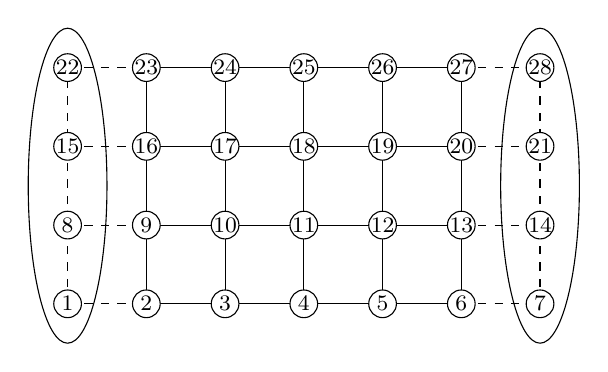
\begin{tikzpicture}[scale = 1.00]
        \draw (1,0) grid  (5,3);
        \draw [dashed] (0,0) grid (1,3);
        \draw [dashed] (5,0) grid (6,3);
        
        \draw (0,1.5) ellipse (.5cm and 2cm);
        \draw (6,1.5) ellipse (.5cm and 2cm);
        
        
        \draw [fill=white] (0,0) circle [radius = 5pt];
        \node     at (0,0) {\footnotesize{1}};
        \draw [fill=white] (1,0) circle [radius = 5pt];
        \node     at (1,0) {\footnotesize{2}};
        \draw [fill=white] (2,0) circle [radius = 5pt];
        \node     at (2,0) {\footnotesize{3}};
        \draw [fill=white] (3,0) circle [radius = 5pt];
        \node     at (3,0) {\footnotesize{4}};
        \draw [fill=white] (4,0) circle [radius = 5pt];
        \node     at (4,0) {\footnotesize{5}};
        \draw [fill=white] (5,0) circle [radius = 5pt];
        \node     at (5,0) {\footnotesize{6}};
        \draw [fill=white] (6,0) circle [radius = 5pt];
        \node     at (6,0) {\footnotesize{7}};

        \draw [fill=white] (0,1) circle [radius = 5pt];
        \node     at (0,1) {\footnotesize{8}};
        \draw [fill=white] (1,1) circle [radius = 5pt];
        \node     at (1,1) {\footnotesize{9}};
        \draw [fill=white] (2,1) circle [radius = 5pt];
        \node     at (2,1) {\footnotesize{10}};
        \draw [fill=white] (3,1) circle [radius = 5pt];
        \node     at (3,1) {\footnotesize{11}};
        \draw [fill=white] (4,1) circle [radius = 5pt];
        \node     at (4,1) {\footnotesize{12}};
        \draw [fill=white] (5,1) circle [radius = 5pt];
        \node     at (5,1) {\footnotesize{13}};
        \draw [fill=white] (6,1) circle [radius = 5pt];
        \node     at (6,1) {\footnotesize{14}};
        
        \draw [fill=white] (0,2) circle [radius = 5pt];
        \node     at (0,2) {\footnotesize{15}};
        \draw [fill=white] (1,2) circle [radius = 5pt];
        \node     at (1,2) {\footnotesize{16}};
        \draw [fill=white] (2,2) circle [radius = 5pt];
        \node     at (2,2) {\footnotesize{17}};
        \draw [fill=white] (3,2) circle [radius = 5pt];
        \node     at (3,2) {\footnotesize{18}};
        \draw [fill=white] (4,2) circle [radius = 5pt];
        \node     at (4,2) {\footnotesize{19}};
        \draw [fill=white] (5,2) circle [radius = 5pt];
        \node     at (5,2) {\footnotesize{20}};
        \draw [fill=white] (6,2) circle [radius = 5pt];
        \node     at (6,2) {\footnotesize{21}};
        
        \draw [fill=white] (0,3) circle [radius = 5pt];
        \node     at (0,3) {\footnotesize{22}};
        \draw [fill=white] (1,3) circle [radius = 5pt];
        \node     at (1,3) {\footnotesize{23}};
        \draw [fill=white] (2,3) circle [radius = 5pt];
        \node     at (2,3) {\footnotesize{24}};
        \draw [fill=white] (3,3) circle [radius = 5pt];
        \node     at (3,3) {\footnotesize{25}};
        \draw [fill=white] (4,3) circle [radius = 5pt];
        \node     at (4,3) {\footnotesize{26}};
        \draw [fill=white] (5,3) circle [radius = 5pt];
        \node     at (5,3) {\footnotesize{27}};
        \draw [fill=white] (6,3) circle [radius = 5pt];
        \node     at (6,3) {\footnotesize{28}};
        
        
    \end{tikzpicture}
    \caption{An example of the grid ordering on an 7 x 4 grid.}
    \label{graph:gridordering}
  \end{center}
\end{figure}


To solve this system, the problem is converted into the form
\begin{equation}
  \mathcal{A} p = b
\end{equation}
where $\mathcal{A}$ is the coefficents for each grid point, $p$ is the solution vector, and $b$ is the boundary conditions. To compute this a bijective mapping to convert the 2D grid into a 1D array is required, the following mapping is used here,
\begin{equation}
  \begin{aligned}
    \pi : \{0,\ldots, n\} \times \{0, \ldots, m \} &\to \{ 1, \ldots, (n+1)(m+1) \} \\
          (i,j) \qquad \qquad &\mapsto  \quad \qquad \pi(i,j)
  \end{aligned}
\end{equation}
An example of this grid ordering can be seen in Figure \ref{graph:gridordering}.

\begin{figure}[h!tb]
  \begin{center}
    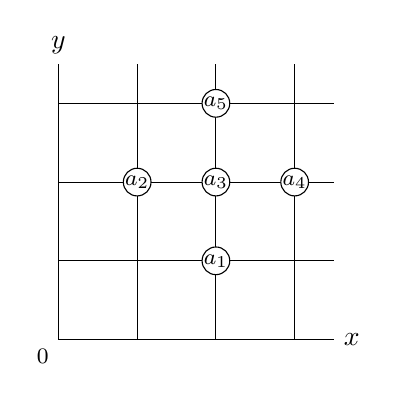
\begin{tikzpicture}[scale = 1.00]
        \draw (-1,-1) grid (1,2.5);
        \draw (1,-1) grid (2.5,2.5);
        
        \node [below left] at (-1,-1) {\footnotesize{0}};
        \node [right] at (2.5,-1) {$x$};
        \node [above] at (-1,2.5) {$y$};
        
        \draw [fill=white] (1,1) circle [radius = 5pt];
        \node at (1,1) {\footnotesize{$a_3$}};
        \draw [fill=white] (0,1) circle [radius = 5pt];
        \node at (0,1) {\footnotesize{$a_2$}};
        \draw [fill=white] (1,0) circle [radius = 5pt];
        \node at (1,0) {\footnotesize{$a_1$}};
        \draw [fill=white] (2,1) circle [radius = 5pt];
        \node at (2,1) {\footnotesize{$a_4$}};
        \draw [fill=white] (1,2) circle [radius = 5pt];
        \node at (1,2) {\footnotesize{$a_5$}};
        
    \end{tikzpicture}
    \caption{A visual of the grid point dependency and their numbering for the diagonally formatted matrix}
    \label{graph:numbering}
  \end{center}
\end{figure}

The matrix is stored in diagonal format and since there are five unknowns for each linear equation the matrix will be banded with five diagonals. The numbering of these diagonals in the matrix can be seen in Figure \ref{graph:numbering} 



\section{Reduce to 1D problem}

  The system (\ref{equ:model_system} - \ref{equ:model_functions}) can be reduced to a $1D$ problem. 
  
  %!% ADD HERE THE BASICS FOR THE TRAVELLING WAVE SCENARIO (HOMOGENOUS IC ON REGION BOUNDARY)
  
  Since the initial conditions are homogenous with respect to x, the x axis can be ignored and only the y-z axis is needed for visualization. Looking at Figure \ref{fig:visual}, the homoginity is clear.
   
  \begin{figure}[h!bt]
    \begin{center}
      \begin{tabular}{c c}
        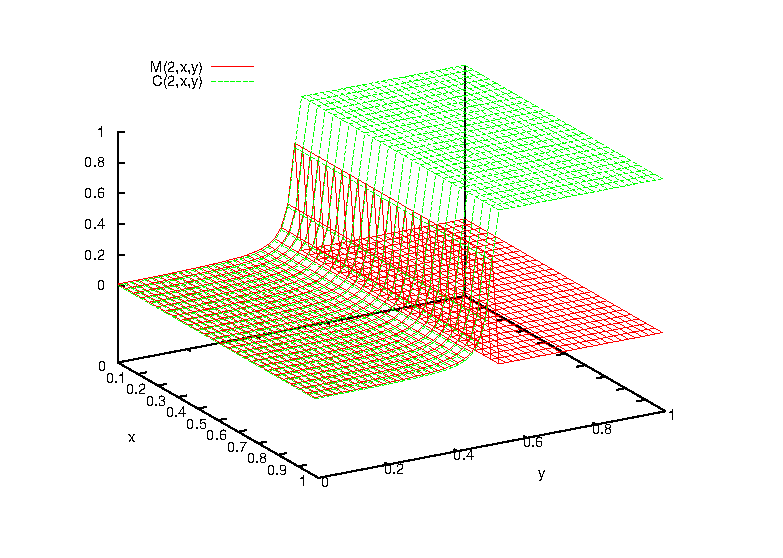
\includegraphics[scale=0.5]{view_3D.eps} &
        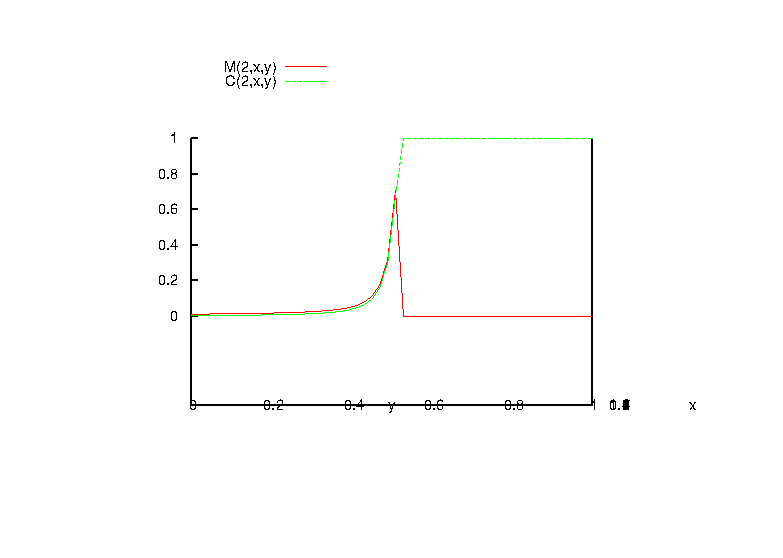
\includegraphics[scale=0.5]{view_psuedo2D.eps} \\
        (a) & (b) \\
      \end{tabular}
      \caption{Graph of (a) 3D view of $M(t,x,y)$ and $C(t,x,y)$, (b) Side profile view of $M(t,x,y)$ and $C(t,x,y)$ at $t=2$.} 
      \label{fig:visual}
    \end{center}
  \end{figure}
   
    This can be shown quantitatily by comparing the maximum and minimum values of M and C with respect to the x-axis (Figure \ref{fig:maxMin}). 
  \begin{figure}[h!bt]
    \begin{center}
        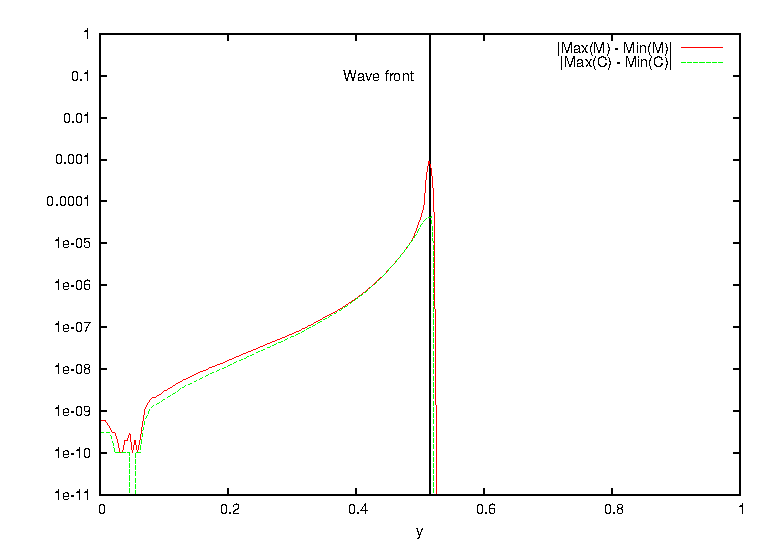
\includegraphics[scale=0.8]{maxMin_MC.eps}
      \caption{Graph of difference between max and min of M and difference between max and min of C.}
      \label{fig:maxMin}
    \end{center}
  \end{figure}

  The difference between the max and min remains constant with respect to time (Table \ref{tab:overTime}), this was calculated by,
  \begin{equation}
    \begin{aligned}
      \delta_M(t) &= \frac{1}{256}\sum_{i = 1}^n \left( \sup_{j \in (1,m)} M(x_i,y_j) - \inf_{k \in (1,m)} M(x_i,y_k) \right) \\
      \delta_C(t) &= \frac{1}{256}\sum_{i = 1}^n \left( \sup_{j \in (1,m)} C(x_i,y_j) - \inf_{k \in (1,m)} C(x_i,y_k) \right)   
    \end{aligned}
  \end{equation}
  
   \begin{table}
    \begin{center}
      \begin{tabular}{| c | c | c |} 
        \hline
        t & $\delta_M$ & $\delta_C$ \\
        \hline
        0.0 & 0.0 & 0.0037109375 \\
        0.5 &1.71577851563e-06 & 0.00371116503633\\
        1.0 &7.62408671875e-06 & 0.00371156747773\\
        1.5 &9.04633828125e-06 & 0.00371216829336\\
        2.0 &7.648728125e-06 & 0.00371311224609\\
        2.5 &2.58707890625e-06 & 0.00371457725742\\
        3.0 &0.00162623974609 & 0.00240237613672\\
        3.5 &5.35270417969e-05 & 7.24265101562e-05\\
        4.5 &1.07250539062e-05 & 2.12679726563e-05 \\
        5.0 &1.09254414063e-06 & 9.720734375e-06\\
        \hline
      \end{tabular}
      \caption{A table of values for $\delta_M(t)$ and $\delta_C(t)$}
      \label{tab:overTime}
    \end{center}
  \end{table}
   
   So by taking the average of the points along the $x$-axis we can get a 2D plot as seen in Figure \ref{fig:true2D}. 
   
 
   
 
    
  \begin{figure}[h!bt]
    \begin{center}
        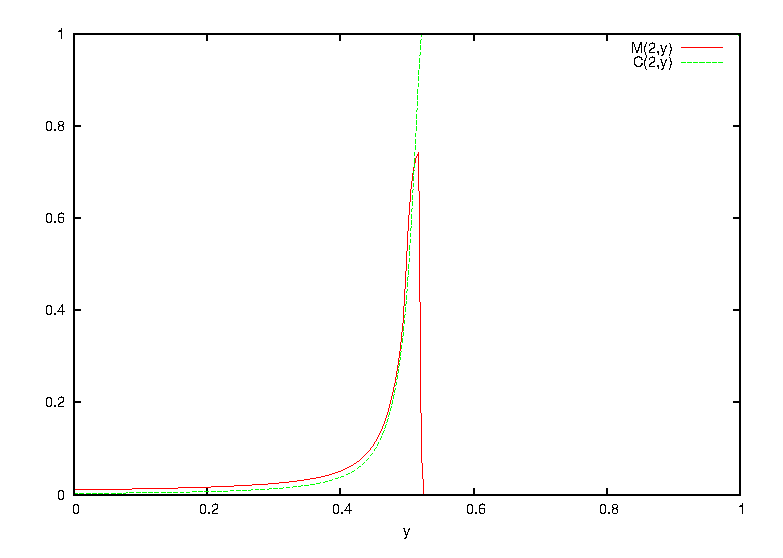
\includegraphics[scale=0.8]{view_2D.eps}
      \caption{Graph of M(2,y) and C(2,y), now reduced to a 2D plot.}
      \label{fig:true2D}
    \end{center}
  \end{figure}








%In here will be the testings and thought process of the convergence results

%In here discuss the extensive testing on how fast computations take and how fine the grid for the finite difference method needs to be so that a sufficient convergence can be observed.

%If I ever get around to it, refere to the results of convergence testing though Python is.

%(Show the results of a convergence analysis.)
%    Maybe use the epsilon delta thing from sci. comp class.
%    Then this section will be mostly an explain of what the epsilon delta 
%        thing and then a few graphs of the different convergence results
%    run the different tests for different t values???

\section{Convergence Results}


The accuracy of this method depends on the grid size used. A convergence analysis is done to observe at what resolution sufficient accuracy is seen. This is done by comparing the relative error in average $M$ between two solutions with different $\Delta x$. We call this difference $\delta$, which we compute as
\begin{equation} \label{equ:converg_delta}
    \delta_k = \frac{\left|\overline{M}_{k+1} - \overline{M}_{k} \right|}{\overline{M}_{k+1}}
\end{equation}
where $\overline{M}_{k}(t)$ is the average biomass at time $t$, solved with $\Delta x = 2^{-k}$. Figure \ref{fig:converg_average} was computed using (\ref{equ:converg_delta}) with $k = 7,8,...,14$. 


\begin{figure}[!htb]
    \begin{center}
        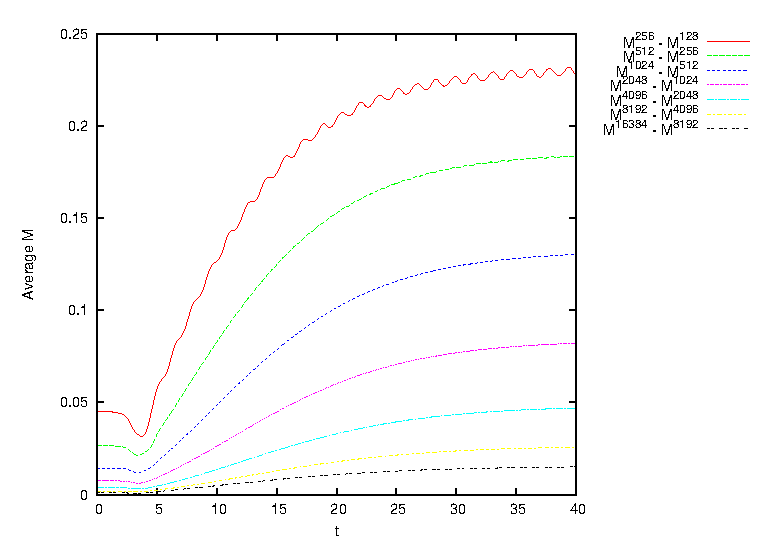
\includegraphics[scale=0.7]{converg_total.eps}
        \caption{Comparison of mean $M$, using (\ref{equ:converg_delta}) with $i = 7,8,...,14$}
        \label{fig:converg_average}
    \end{center}
\end{figure}

This convergence analysis shows a relative error less then $0.02\%$ can be achieved by using $\Delta x = 2^{-13}$. This is considered an sufficient accuracy.
%!%
%!%
%!% FIND A SOURCE THAT SAYS THIS IS ACCURATE ENOUGH
%!%
%!%

A second convergence result can be done by instead comparing each gridpoint between solutions. If we define 
\begin{equation} \label{equ:converg_sigma}
    \sigma_k(t) = 2^{-k} \sum_{i,j} |M^{k+1}(t, x_i, y_j) - M^k(t, x_i, y_i)|,
\end{equation}
and 
\begin{equation} \label{equ:converg_rho}
    \rho_k = \frac{1}{n(T)} \sum_{\forall t \in T} \sigma_k(t).
\end{equation}
In (\ref{equ:converg_sigma}), $M^{k}(t,x_i,y_i)$ refers to the biomass when solved with $\Delta x = 2^{-k}$ at time t and gridpoint $(x_i, y_i)$. The value of $\sigma_k(t)$ is the average difference between related gridpoints of solutions solved with different $\Delta x$ values at a specific time $t$. In (\ref{equ:converg_rho}), $n(T)$ refers to the cardinality of $T$, which is the number of outputted times we have. The value of $\rho$ is the average difference across all $t \in T$. 
%!% Reference the nonexistance figure here.

\begin{figure}[!htb]
    \begin{center}
  %!% Make this figure exist      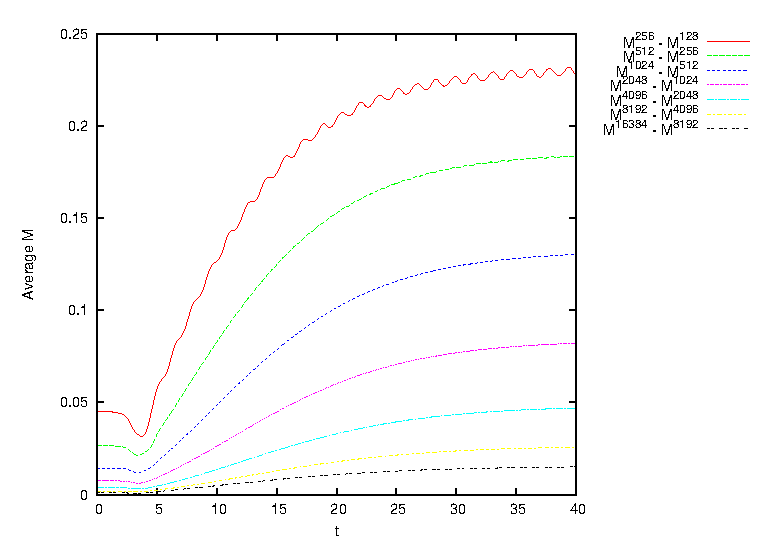
\includegraphics[scale=0.7]{converg_total.eps}
        \caption{Graph of $\rho_k$, for $k = 7,8,...,13$ and $T = 0,2,...,40$}
        \label{fig:converg_rho}
    \end{center}
\end{figure}

This can be extended to check convergence in $\Delta t$ by defining
\begin{equation} \label{equ:converg_rhoBar}
    \overline{\rho}_{\tau} = \sum_k \rho^{\tau}_k
\end{equation}
where $\rho^{\tau}_k$ is the same computations for (\ref{equ:converg_rho}) done with $\Delta t = \tau$.

%!% Add a table of values for \rho^{\tau}







%\section{Typical Simulation}
Is Typical\_simulation.tex needed in this section?
If anything it would be the sanity check simulations


The system
  \begin{align}
    M_t &= \nabla_x \left( D(M) \nabla_x M \right) + f(C,M) M \\
    C_t &= - g(C,M) 
  \end{align}
  where
  \begin{align}
    D(M) &= \delta \frac{M^\alpha}{(1 - M)^\beta} \\
    f(C,M) &= \frac{ C }{{k } + {C}} \left(1 - \left( \frac{M M_0}{{C C_0 + \epsilon}} \right)^\gamma \right) \\
    g(C,M) &= \frac{\nu C}{k +C} M
  \end{align}
  is solved on a rectangular region with length $L$ and width $\lambda L$ with the following parameter values,
  \begin{equation}
    \begin{aligned}
      L &= 0.01 \\
      \lambda &= \frac{1}{128}\\
      \epsilon &= 10^{-8}\\
      \alpha &= 4 \\
      \beta &= 4 \\
      \gamma &= 0.5 \\
      \mu &= 6 \\      
    \end{aligned}
    \qquad
    \begin{aligned}
      C_0 &= 30 \\
      M_0 &= 30 \\
      \delta &= \frac{10^{-7}}{\mu L^2} \approx 10^-4\\
      k &= \frac{4}{C_0} \approx 0.1333\\
      \nu &= \frac{M_0}{0.63 C_0} \approx 1.59,\\
    \end{aligned}
  \end{equation}
  and with initial conditions 
  \begin{equation}
    \begin{aligned}
      C &= 1 \\
      M &= \begin{cases} -(\frac{h}{d^4})x^4 + h & \text{if } x < 0.04 \\ 0 & \text{otherwise }\end{cases} \\
    \end{aligned}
  \end{equation}  
  where $h = 0.05, d=0.04$ , representing the height and depth of the inoculation site.

  A series of test was done on simulation code version $0.1.1$. These were defaulted to run with $\Delta t = 10^{-3}$ and $\Delta x = \frac{1}{256}$.
  
  The following lists the test, and observations from each.
  
  \begin{enumerate}
    \item Solve the system with homogenous initial conditions and see if it stays homogenous.
      \begin{itemize}
        \item Worked!
        \item The biomass and substrate concentration at $t=8$ did not change as grid size did, which is good. 
        \item Biomass and substrate concentration did change for step size, but it was converging to a specific value (Table \ref{tab:homoIC}), which makes sense and suggests that default choice of $\Delta t$ is good.
        \begin{table}
          \begin{center}
            \begin{tabular}{| c | c | c |}
              \hline
              $\Delta t$ & Biomass Density & Substrait Conc. \\
              \hline
              $10^{-1}$ & 0.743806469443 & 0.731575100108\\
              $10^{-2}$ & 0.739180637812 & 0.736539504220\\
              $10^{-3}$ & 0.738699851204 & 0.737025027162 \\
              $10^{-4}$ & 0.738651598939 & 0.737073472750\\
              $10^{-5}$ & 0.738646771985 & 0.737078316244\\
              \hline
            \end{tabular}
            \caption{Values of biomass and substrate concentration at $t = 8$. A grid size of $\Delta x = 1/256$ was used.}
            \label{tab:homoIC}
          \end{center}
        \end{table}
      \end{itemize}

%    \item Solve the system with non-homogenous high initial condition ($M_0=0.95$), with zero forcing term, and see if density-dependent diffusion moves it without loss of biomass.
%      \begin{itemize}
%        \item DOESN"T WORK!!!!!!
%      \end{itemize}
  
      
    \item Solve the system with $f = s$, $s$ a constant, and see if total biomass follows $be^{st}$, where $b$ is the initial total biomass.
    \begin{itemize}
      \item Works with $D(M) = 0$.
      
      \item With $D(M) = \delta$ total biomass grows a little slower then $be^{st}$ which becomes slightly noticable at later times. The difference is less then 1\%, so this looks good. See Figure \ref{fig:totalBioCheck}(ab).
      
      \item With $D(M) = \delta M^{\alpha}$ the total biomass matchs $be^{st}$ until the biomass density at the innoculation point becomes greater then 1. Since physically this should never occur, this isn't a problem.  See Figure \ref{fig:totalBioCheck}(c).
      
      \item With $D(M) = \frac{\delta M^{\alpha}}{(1-M)^\beta}$ the total biomass grows accuratly until it approches $M \in (0.9, 1)$ at the innoculation point. This is a problem, because at this point the density dependent diffusion should start and keep the solution growing with $be^{st}$. This suggests that there is something wrong with how the diffusion is being implemented, will follow up on this.  See Figure \ref{fig:totalBioCheck}(d).
      
      \begin{figure}
        \begin{center}
          \begin{tabular}{c c}
            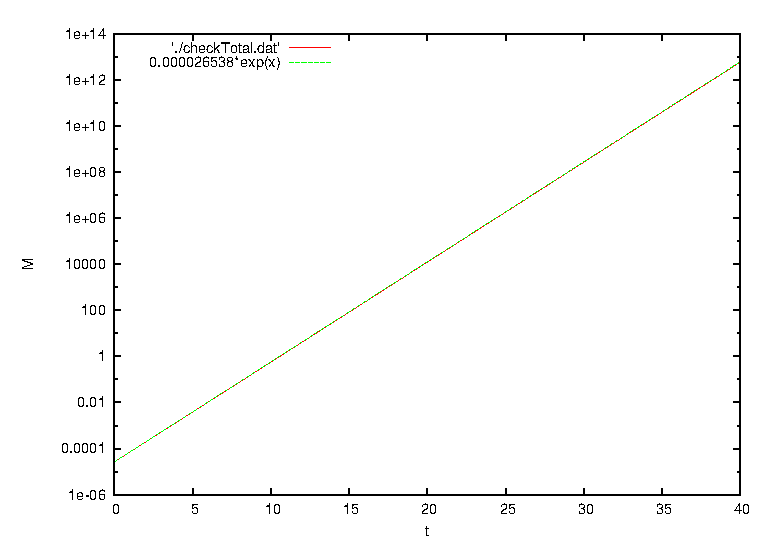
\includegraphics[scale=0.5]{checkTotal_Dconstant.eps} &
            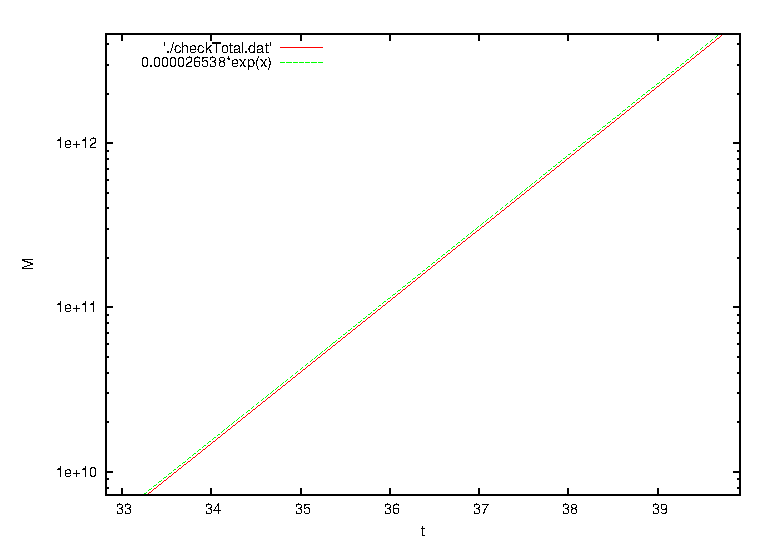
\includegraphics[scale=0.5]{checkTotal_Dconstant_zoomed.eps} \\
            (a) & (b) \\
            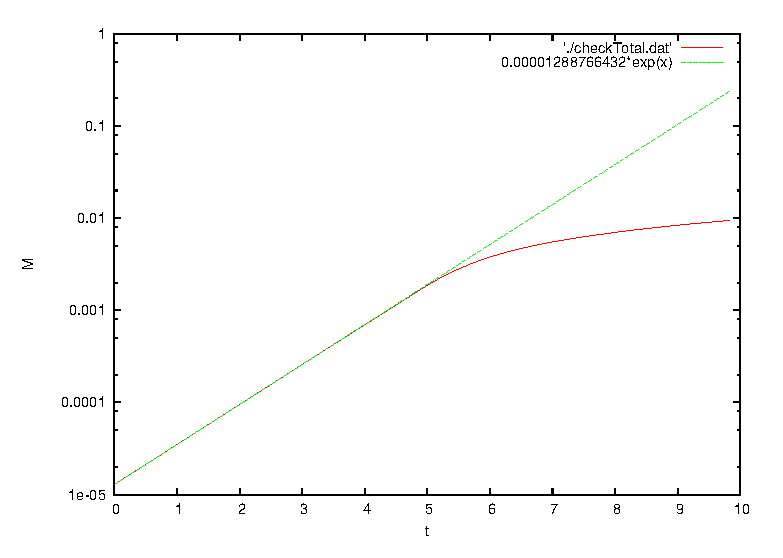
\includegraphics[scale=0.5]{checkTotal_Dporous.eps} & 
            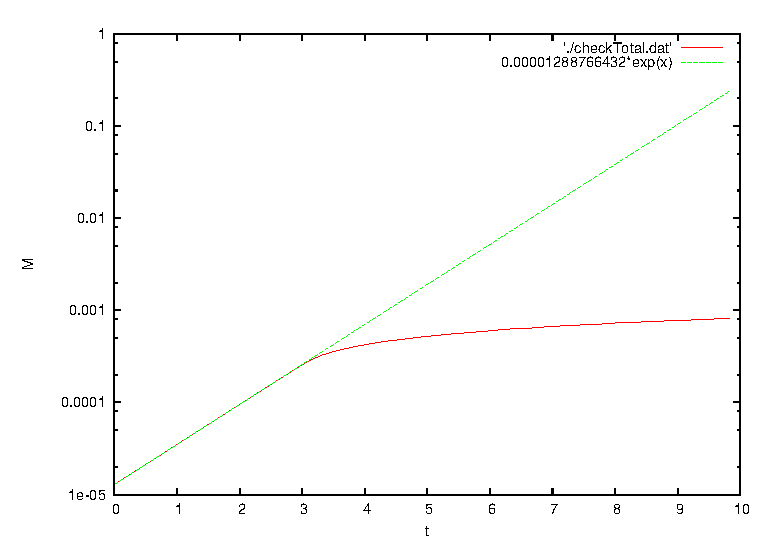
\includegraphics[scale=0.5]{checkTotal_Ddensity.eps} \\
            (c) & (d) \\
          \end{tabular}
          \captionsetup{singlelinecheck=off}
          \caption[enum]{Graph of, 
            \begin{enumerate}[(a)]
              \item $D(M) = \delta$, 
              \item $D(M) = \delta$; zoomed in to show the slight difference in growth,
              \item $D(M) = \delta M^\alpha$,
              \item $D(M) = \frac{\delta M^{\alpha}}{(1-M)^\beta} $.
            \end{enumerate} 
          }

          \label{fig:totalBioCheck}
        \end{center}
      \end{figure}
      
    \end{itemize}
      
  \end{enumerate}

\section{Iterations}

In here will be the description of the method and results of iterating between solvings of M and C until the difference has convergenced to a a specificed epsilon. Also mention in here the effects it has on the solutions (not much) and computation time (2x longer ish?). Also discuss the single iterations and its effects (solve M -> solve C -> solve M again).


  The system
  \begin{align}
    M_t &= \nabla_x \left( D(M) \nabla_x M \right) + f(C,M) M \\
    C_t &= - g(C,M) 
  \end{align}
  where
  \begin{align}
    D(M) &= \delta \frac{M^\alpha}{(1 - M)^\beta} \\
    f(C,M) &= \frac{ C }{{k } + {C}} \left(1 - \left( \frac{M M_0}{{C C_0 + \epsilon}} \right)^\gamma \right) \\
    g(C,M) &= \frac{\nu C}{k +C} M
  \end{align}
  is solved on a rectangular region with length $L$ and width $\lambda L$ with the following parameter values,
  \begin{equation}
    \begin{aligned}
      L &= 0.01 \\
      \lambda &= \frac{1}{128}\\
      \epsilon &= 10^{-8}\\
      \alpha &= 4 \\
      \beta &= 4 \\
      \gamma &= 0.5 \\
      \mu &= 6 \\      
    \end{aligned}
    \qquad
    \begin{aligned}
      C_0 &= 30 \\
      M_0 &= 30 \\
      \delta &= \frac{10^{-7}}{\mu L^2} \approx 10^-4\\
      k &= \frac{4}{C_0} \approx 0.1333\\
      \nu &= \frac{M_0}{0.63 C_0} \approx 1.59,\\
    \end{aligned}
  \end{equation}
  and with initial conditions 
  \begin{equation}
    \begin{aligned}
      C &= 1 \\
      M &= \begin{cases} -(\frac{h}{d^4})x^4 + h & \text{if } x < 0.04 \\ 0 & \text{otherwise }\end{cases} \\
    \end{aligned}
  \end{equation}  
  where $h = 0.1, d=\frac{5}{128}$ , representing the height and depth of the inoculation site.

  Using simulation code version $0.4$ the effect of iterating between solving $M$ and $C$ was examined. Algorithm \ref{alg:iterateCM} shows how the iterations was implemented. The following experiments were run on the simulator.
  
  \begin{algorithm}[h!tb]
      \dontprintsemicolon
      \KwData{eSoln = $10^{-12}$; $M_{prev}$ and $C_{prev}$ is previous timestep solutions}
      \Begin
      {
        \SetLine
        \While{diffC + diffM  $> $ eSoln}
        {
            Solve for $M^{i+1}$ using $C^{i}$ and $M_{prev}$\;
            Solve for $C^{i+1}$ using $C_{prev}$, $M^{i+1}$, and $M_{prev}$\;
            Let diffC $=  (C^{i+1} - C^i)$\;
            Let diffM $= (M^{i+1} - M^i)$\;
            Let $C^{i} = C^{i+1}$\;
            Let $M^{i} = M^{i+1}$\;
        }
      }
      \caption{Algorithm for iterating between solutions.}
      \label{alg:iterateCM}
    \end{algorithm}
  
  Figure \ref{fig:iterateAccuracy} shows how the error between the iterated solutions changes the solutions. Notice that there is very little difference.
  
  \begin{figure}[h!tb]
    \begin{center}
      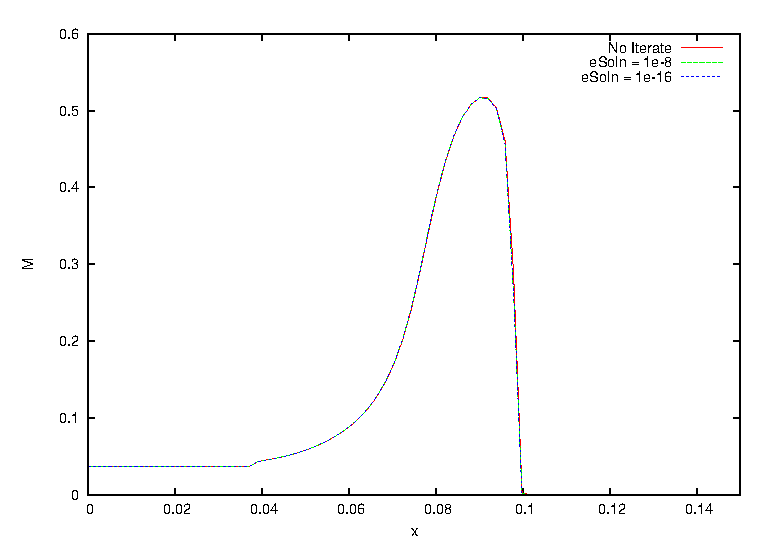
\includegraphics[scale=0.85]{eSolnCheck.eps}
      \caption{Convergence of solutions for no iterations between solutions, or iterating with different accuracy values.}
      \label{fig:iterateAccuracy}
    \end{center}
  \end{figure}
  
    
  Figure \ref{fig:convergeDelt} shows, for different $\Delta t$ values, the convergence of solutions as $\Delta x$ becomes smaller. Very minute differences between $\Delta t$ values.
  
  \begin{figure}[h!tb]
    \begin{center}
      \begin{tabular}{c c}
          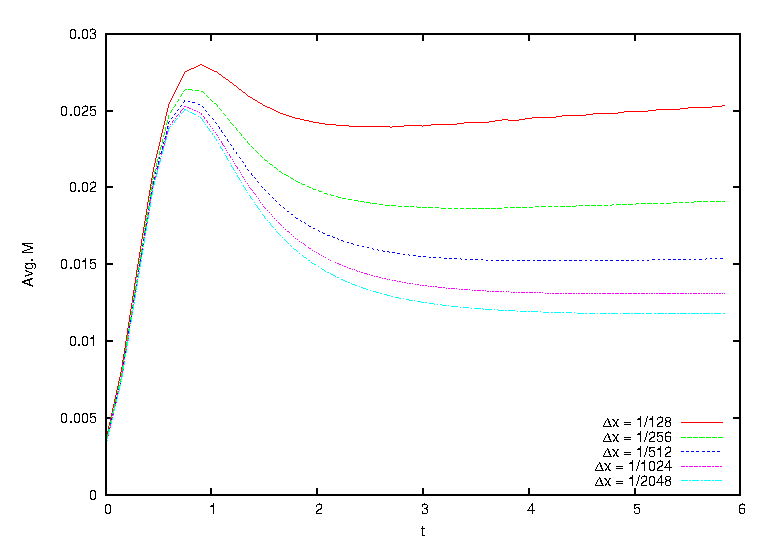
\includegraphics[scale=0.55]{converge_tDel1e-2.eps} &
          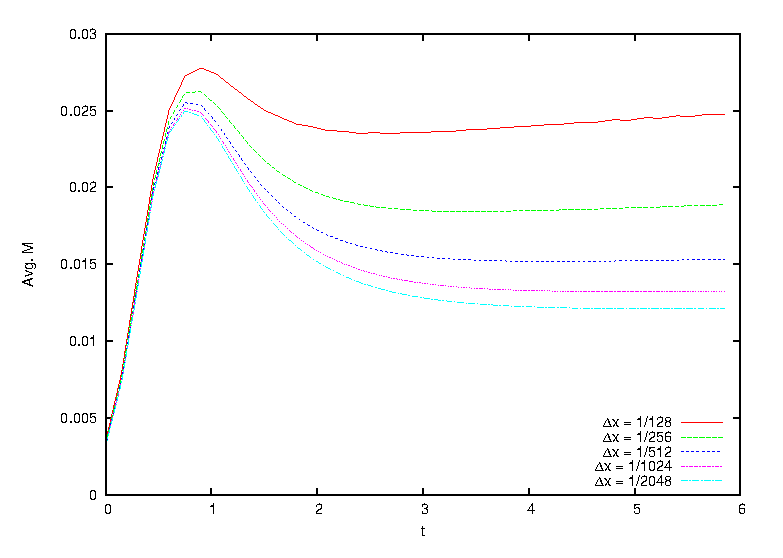
\includegraphics[scale=0.55]{converge_tDel1e-3.eps} \\
          (a) & (b) \\
          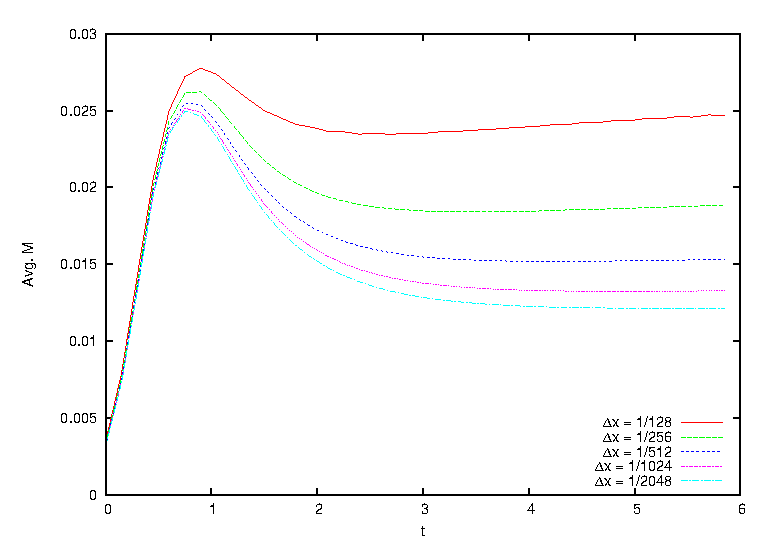
\includegraphics[scale=0.55]{converge_tDel1e-4.eps} & \\
          %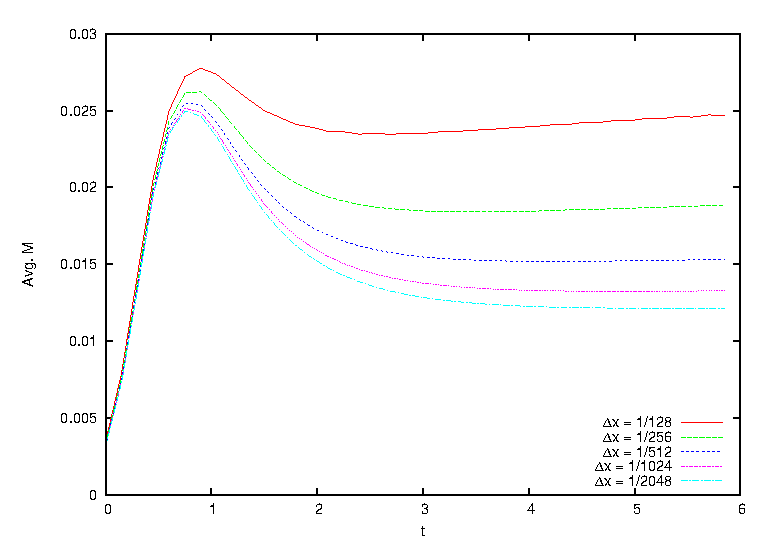
\includegraphics[scale=0.8]{converge_tDel1e-4.eps} \\
          (c) & (d)
      \end{tabular}
      \caption{Convergence of solutions for (a) $\Delta t = 10^{-2}$, (b) $\Delta t = 10^{-3}$, (c) $\Delta t = 10^{-4}$, (d) $\Delta t = 10^{-5}$.}
      \label{fig:convergeDelt}
    \end{center}
  \end{figure}
  
   Figure \ref{fig:functionC} shows the convergence of solutions if the computation of $M$ depends on a arbitrary function, $\hat{C}$, instead of the substrait concentration. 
  
  \begin{figure}[h!tb]
    \begin{center}
      \begin{tabular}{c c}
          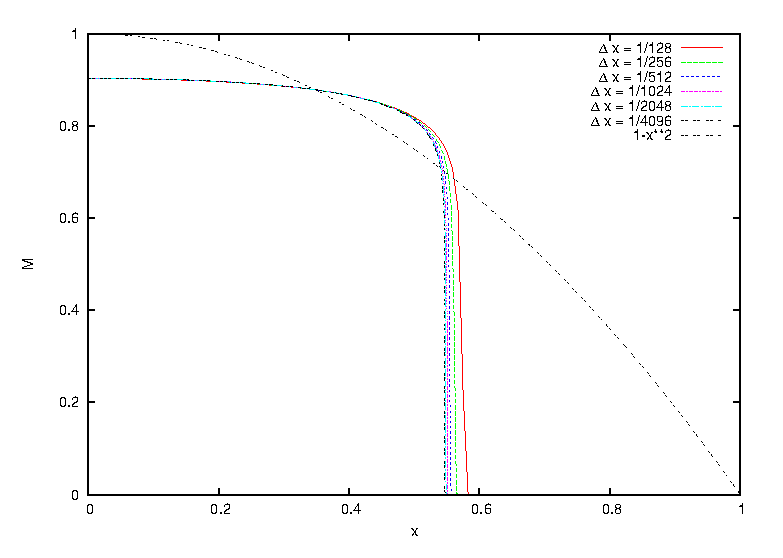
\includegraphics[scale=0.55]{Cfunc_polynomial_t=5-25.eps} &
          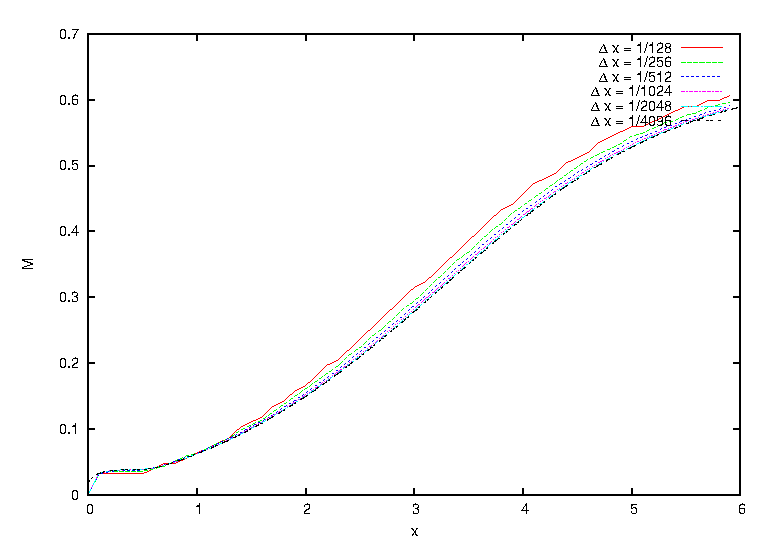
\includegraphics[scale=0.55]{Cfunc_polynomial_interface.eps} \\
          (a) & (b) 
      \end{tabular}
      \caption{Convergence of solutions for $\hat{C}(x) = 1-x^2$ looking at (a) solutions at $t = 5.25$ and (b) the interface x position.}
      \label{fig:functionC}
    \end{center}
  \end{figure}
  
   Figure \ref{fig:kinematics} show how the solutions converge for different functions $f(C,M)$. Some of which do not depend on $C$ or $M$. 
  
  \begin{figure}[h!tb]
    \begin{center}
      \begin{tabular}{c c}
          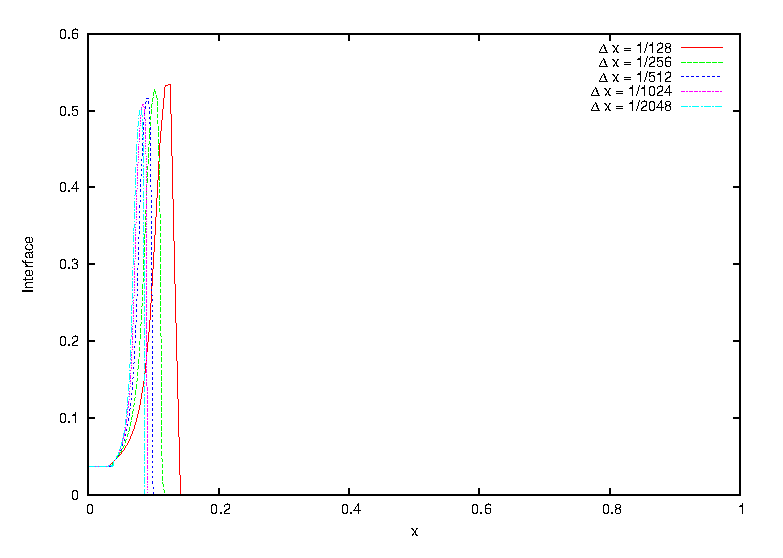
\includegraphics[scale=0.55]{Fdefault.eps} &
          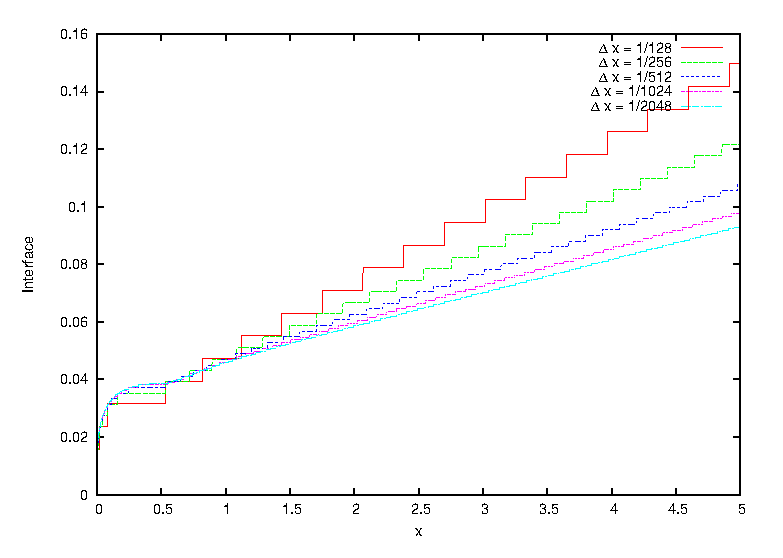
\includegraphics[scale=0.55]{FdefaultInterface.eps} \\
          (a) & (b) \\
          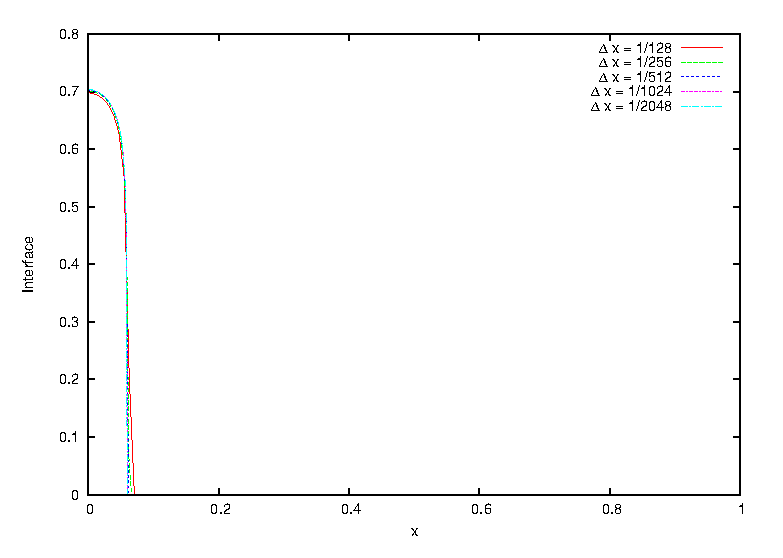
\includegraphics[scale=0.55]{Flogistic_t=4-25.eps} &
          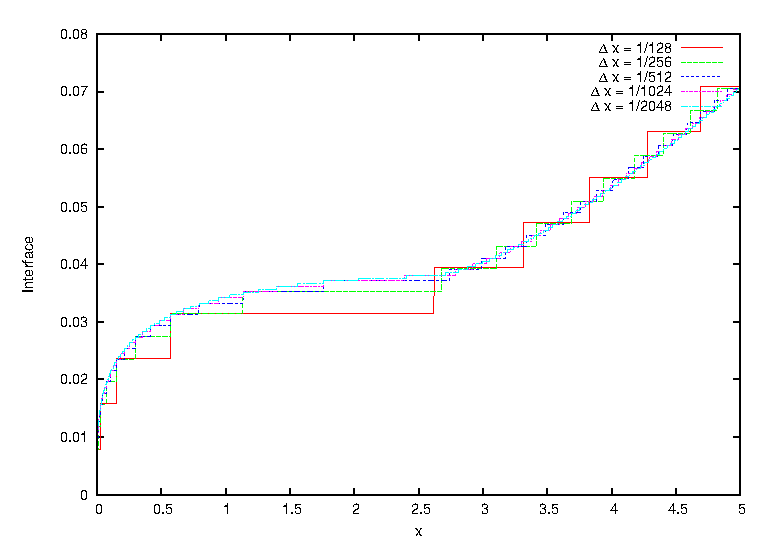
\includegraphics[scale=0.55]{Flogistic.eps} \\
          (c) & (d) \\
          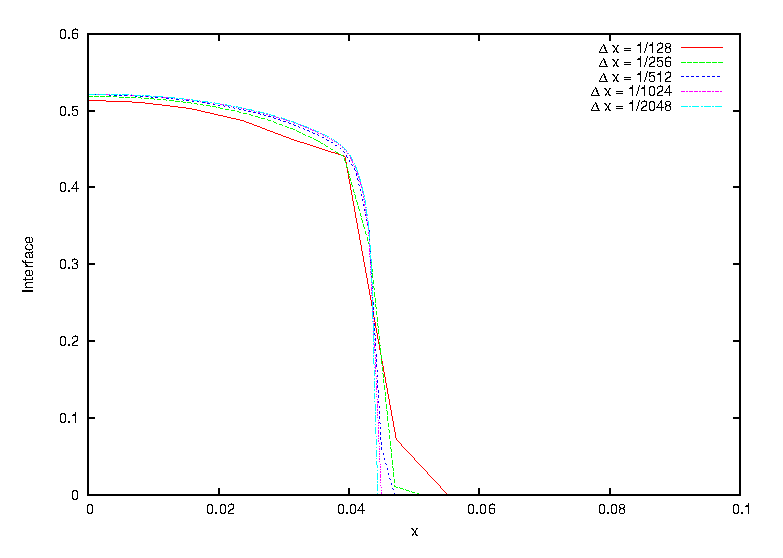
\includegraphics[scale=0.55]{FnoM.eps} &
          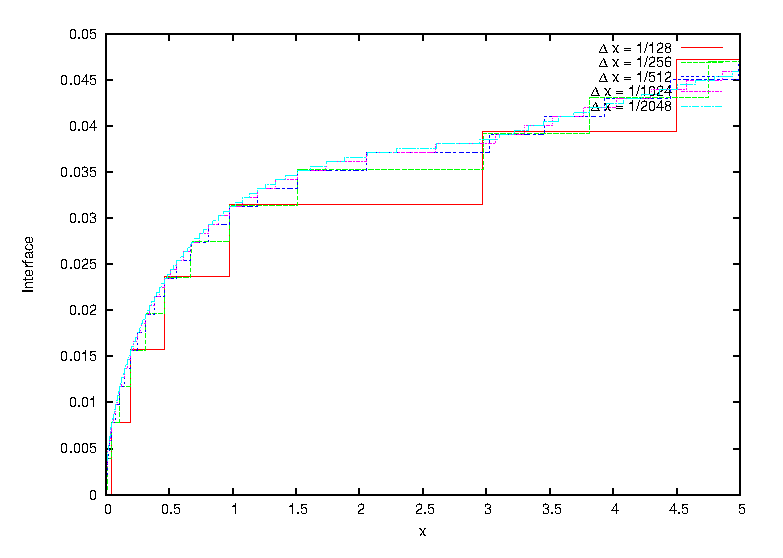
\includegraphics[scale=0.55]{FnoMInterface.eps} \\
          (e) & (f) \\
          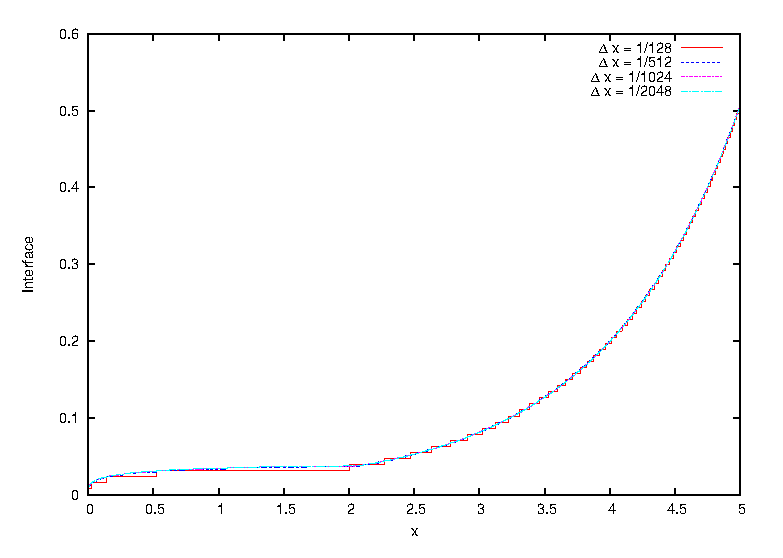
\includegraphics[scale=0.55]{Fconstant.eps} & \\
          (g) & \\ 
      \end{tabular}
      \caption{Convergence of solutions for (a-b) $f(C,M) = $default,  (c-d) $f(C,M) = (1 - M)$, (e-f) $f(C,M) = (1 - C) \frac{C}{M+\epsilon}, $(g) $f(C,M) = 1$. Each pair of graphs is the solution at $t = 4.25$ and the interface as a function of t.}
      \label{fig:kinematics}
    \end{center}
  \end{figure}



\chapter{Simulation Results}
\section{Typical Simulation}
Is Typical\_simulation.tex needed in this section?
If anything it would be the sanity check simulations


The system
  \begin{align}
    M_t &= \nabla_x \left( D(M) \nabla_x M \right) + f(C,M) M \\
    C_t &= - g(C,M) 
  \end{align}
  where
  \begin{align}
    D(M) &= \delta \frac{M^\alpha}{(1 - M)^\beta} \\
    f(C,M) &= \frac{ C }{{k } + {C}} \left(1 - \left( \frac{M M_0}{{C C_0 + \epsilon}} \right)^\gamma \right) \\
    g(C,M) &= \frac{\nu C}{k +C} M
  \end{align}
  is solved on a rectangular region with length $L$ and width $\lambda L$ with the following parameter values,
  \begin{equation}
    \begin{aligned}
      L &= 0.01 \\
      \lambda &= \frac{1}{128}\\
      \epsilon &= 10^{-8}\\
      \alpha &= 4 \\
      \beta &= 4 \\
      \gamma &= 0.5 \\
      \mu &= 6 \\      
    \end{aligned}
    \qquad
    \begin{aligned}
      C_0 &= 30 \\
      M_0 &= 30 \\
      \delta &= \frac{10^{-7}}{\mu L^2} \approx 10^-4\\
      k &= \frac{4}{C_0} \approx 0.1333\\
      \nu &= \frac{M_0}{0.63 C_0} \approx 1.59,\\
    \end{aligned}
  \end{equation}
  and with initial conditions 
  \begin{equation}
    \begin{aligned}
      C &= 1 \\
      M &= \begin{cases} -(\frac{h}{d^4})x^4 + h & \text{if } x < 0.04 \\ 0 & \text{otherwise }\end{cases} \\
    \end{aligned}
  \end{equation}  
  where $h = 0.05, d=0.04$ , representing the height and depth of the inoculation site.

  A series of test was done on simulation code version $0.1.1$. These were defaulted to run with $\Delta t = 10^{-3}$ and $\Delta x = \frac{1}{256}$.
  
  The following lists the test, and observations from each.
  
  \begin{enumerate}
    \item Solve the system with homogenous initial conditions and see if it stays homogenous.
      \begin{itemize}
        \item Worked!
        \item The biomass and substrate concentration at $t=8$ did not change as grid size did, which is good. 
        \item Biomass and substrate concentration did change for step size, but it was converging to a specific value (Table \ref{tab:homoIC}), which makes sense and suggests that default choice of $\Delta t$ is good.
        \begin{table}
          \begin{center}
            \begin{tabular}{| c | c | c |}
              \hline
              $\Delta t$ & Biomass Density & Substrait Conc. \\
              \hline
              $10^{-1}$ & 0.743806469443 & 0.731575100108\\
              $10^{-2}$ & 0.739180637812 & 0.736539504220\\
              $10^{-3}$ & 0.738699851204 & 0.737025027162 \\
              $10^{-4}$ & 0.738651598939 & 0.737073472750\\
              $10^{-5}$ & 0.738646771985 & 0.737078316244\\
              \hline
            \end{tabular}
            \caption{Values of biomass and substrate concentration at $t = 8$. A grid size of $\Delta x = 1/256$ was used.}
            \label{tab:homoIC}
          \end{center}
        \end{table}
      \end{itemize}

%    \item Solve the system with non-homogenous high initial condition ($M_0=0.95$), with zero forcing term, and see if density-dependent diffusion moves it without loss of biomass.
%      \begin{itemize}
%        \item DOESN"T WORK!!!!!!
%      \end{itemize}
  
      
    \item Solve the system with $f = s$, $s$ a constant, and see if total biomass follows $be^{st}$, where $b$ is the initial total biomass.
    \begin{itemize}
      \item Works with $D(M) = 0$.
      
      \item With $D(M) = \delta$ total biomass grows a little slower then $be^{st}$ which becomes slightly noticable at later times. The difference is less then 1\%, so this looks good. See Figure \ref{fig:totalBioCheck}(ab).
      
      \item With $D(M) = \delta M^{\alpha}$ the total biomass matchs $be^{st}$ until the biomass density at the innoculation point becomes greater then 1. Since physically this should never occur, this isn't a problem.  See Figure \ref{fig:totalBioCheck}(c).
      
      \item With $D(M) = \frac{\delta M^{\alpha}}{(1-M)^\beta}$ the total biomass grows accuratly until it approches $M \in (0.9, 1)$ at the innoculation point. This is a problem, because at this point the density dependent diffusion should start and keep the solution growing with $be^{st}$. This suggests that there is something wrong with how the diffusion is being implemented, will follow up on this.  See Figure \ref{fig:totalBioCheck}(d).
      
      \begin{figure}
        \begin{center}
          \begin{tabular}{c c}
            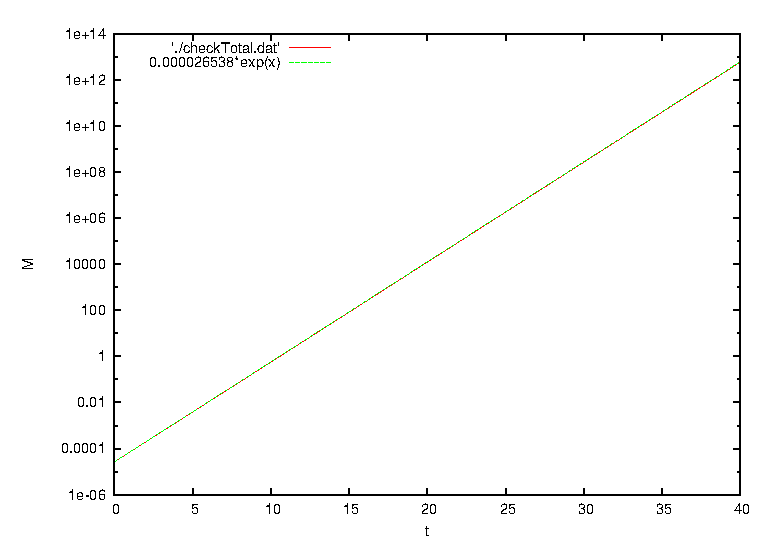
\includegraphics[scale=0.5]{checkTotal_Dconstant.eps} &
            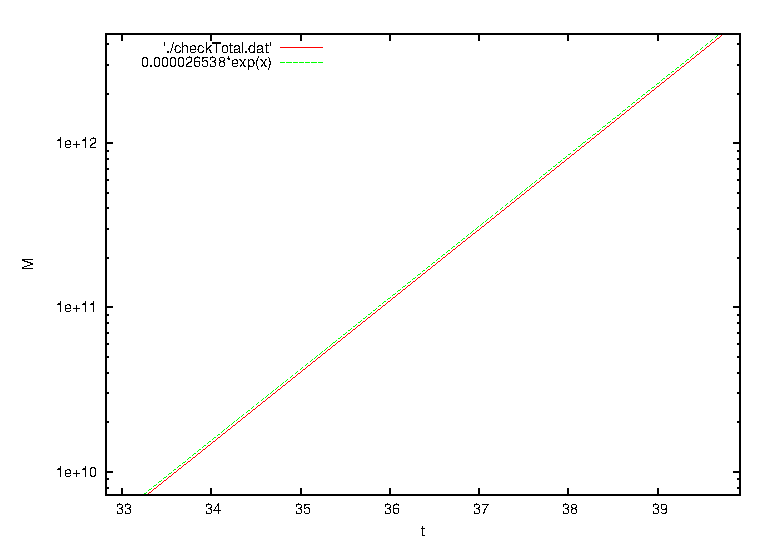
\includegraphics[scale=0.5]{checkTotal_Dconstant_zoomed.eps} \\
            (a) & (b) \\
            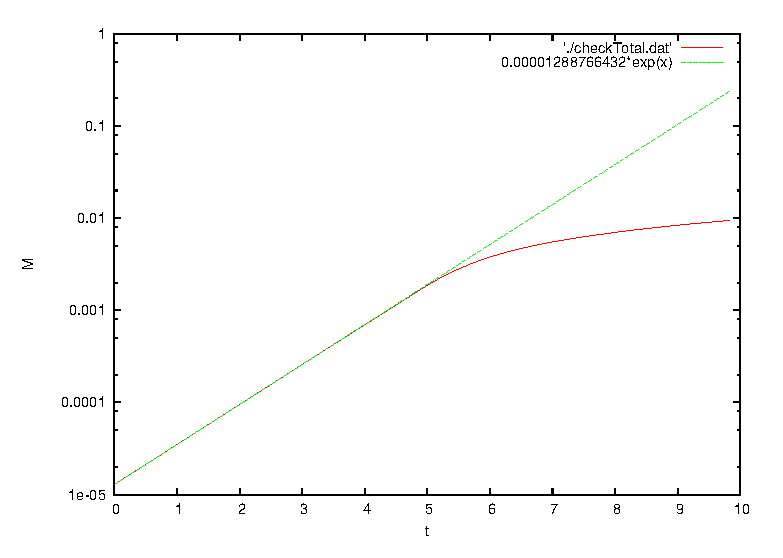
\includegraphics[scale=0.5]{checkTotal_Dporous.eps} & 
            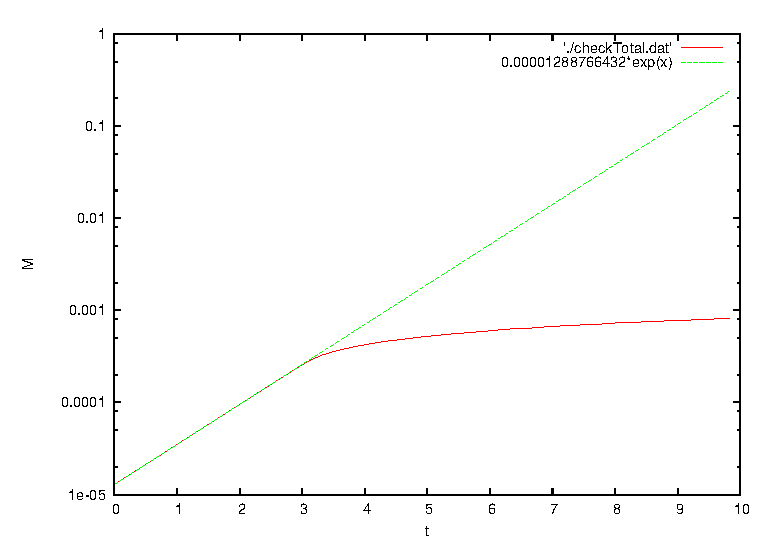
\includegraphics[scale=0.5]{checkTotal_Ddensity.eps} \\
            (c) & (d) \\
          \end{tabular}
          \captionsetup{singlelinecheck=off}
          \caption[enum]{Graph of, 
            \begin{enumerate}[(a)]
              \item $D(M) = \delta$, 
              \item $D(M) = \delta$; zoomed in to show the slight difference in growth,
              \item $D(M) = \delta M^\alpha$,
              \item $D(M) = \frac{\delta M^{\alpha}}{(1-M)^\beta} $.
            \end{enumerate} 
          }

          \label{fig:totalBioCheck}
        \end{center}
      \end{figure}
      
    \end{itemize}
      
  \end{enumerate}

\chapter{Discussions}
Lots of discussion on the things that were analysied in this thesis.

\chapter{Conclusions}
There will be lots of concluding statements in here.


\newpage
\pagestyle{References}
\chapter*{References}
\addcontentsline{toc}{chapter}{\hspace{16pt} Complete Bibliography}
\titlespacing{\section}{0pt}{*0}{*0}
\renewcommand{\bibname}{}
\renewcommand\bibsection{}
\titlespacing{\chapter}{0pt}{*0}{*0}
\titlespacing{\section}{0pt}{*0}{*0}
\setlength{\parskip}{0pt}
\setlength{\parsep}{0pt}
\nocite*
\bibliographystyle{plainnat}
\bibliography{ThesisReferences}



\newpage
\pagestyle{fancy}

%%Appendix A Behavioural Plots Simulation Study
%\input{BackMatter/AppendixA}


\newpage
\thispagestyle{custom}
\mbox{}


\end{document}
